%%%%%%%%%%%%%%%%%%%%%%%%%%%%% Define Article %%%%%%%%%%%%%%%%%%%%%%%%%%%%%%%%%%
\documentclass{article}
%%%%%%%%%%%%%%%%%%%%%%%%%%%%%%%%%%%%%%%%%%%%%%%%%%%%%%%%%%%%%%%%%%%%%%%%%%%%%%%

%%%%%%%%%%%%%%%%%%%%%%%%%%%%% Using Packages %%%%%%%%%%%%%%%%%%%%%%%%%%%%%%%%%%
\usepackage[utf8]{inputenc}
\usepackage[T1]{fontenc}
\usepackage{textcomp}
\usepackage{lmodern}
\usepackage{upquote}
\usepackage[spanish]{babel}
\usepackage{geometry}
\usepackage{graphicx}
\usepackage{float}
\usepackage{amssymb}
\usepackage{amsmath}
\usepackage{amsthm}
\usepackage{empheq}
\usepackage{mdframed}
\usepackage{booktabs}
\usepackage{color}
\usepackage{psfrag}
\usepackage{pgfplots}
\usepackage{bm}
\usepackage{hyperref}
\usepackage{fancyvrb}
\usepackage[label=corner]{karnaugh-map}
%%%%%%%%%%%%%%%%%%%%%%%%%%%%%%%%%%%%%%%%%%%%%%%%%%%%%%%%%%%%%%%%%%%%%%%%%%%%%%%

%%%%%%%%%%%%%%%%%%%%%%%%%% Page Setting %%%%%%%%%%%%%%%%%%%%%%%%%%%%%%%%%%%%%%%
\geometry{a4paper, margin=2.5cm}

%%%%%%%%%%%%%%%%%%%%%%%%%%%%%%% Title & Author %%%%%%%%%%%%%%%%%%%%%%%%%%%%%%%%
\title{Tarea 2: ejertitación para parcial}
\author{Cortesini Perez Luciano Tomas}
\date{Mayo 2026}
%%%%%%%%%%%%%%%%%%%%%%%%%%%%%%%%%%%%%%%%%%%%%%%%%%%%%%%%%%%%%%%%%%%%%%%%%%%%%%%

\begin{document}
\maketitle

\section{Consigna}

\begin{itemize}
    \item Obtener la mínima expresión booleana.
    \item Simular en falstad, (o cualquier simulador).
    \item Describir en verilog.
    \item Presentar la descripción.
    \item Capturar imagen del RTL.
    \item Capturar la simulación temporal.
\end{itemize}

\section{Ejercicio 1}

$$
F(x,y,z) = \sum(2,3,4,5)
$$

\subsection{Expresión mínima}

\begin{figure}[H]
    \centering
    \begin{karnaugh-map}[2][4][1][$z$][$y$][$x$]
        \centering
        \minterms{2,3,4,5}
        \implicant{2}{3}
        \implicant{4}{5}
    \end{karnaugh-map}
    \caption{Mapa de Karnaugh para la función}
\end{figure}

$$
F(x,y,z) = x \overline{y} + \overline{x} y
$$

\subsection{Simulación en Falstad}
\begin{figure}[H]
    \centering
    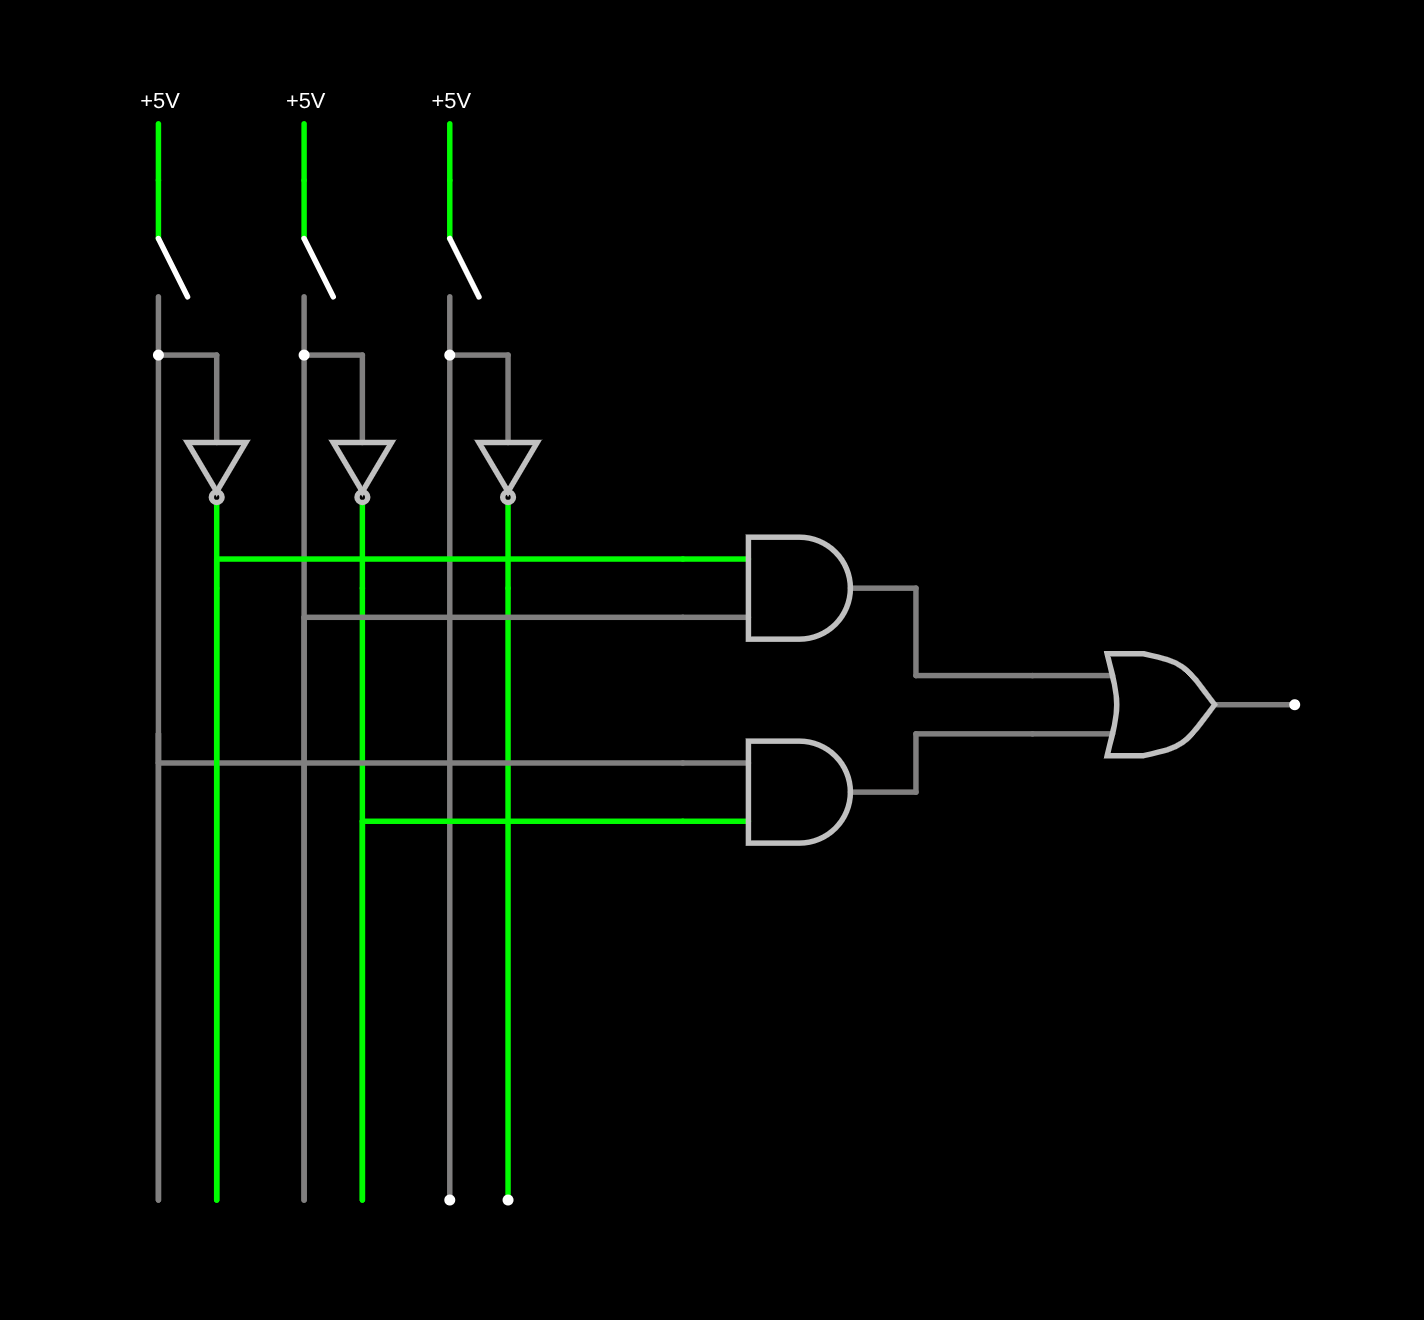
\includegraphics[width=0.6\textwidth]{img/Falstad/ej1.png}
    \caption{Simulación de la función en Falstad}
\end{figure}

\subsection{Descripción en Verilog}

\begin{Verbatim}[ frame=single, fontsize=\small, baselinestretch=1.2 ]
module ej1 (
    input x,
    input y,
    input z,
    output F
);

assign F = x & ~y | ~x & y;

endmodule
\end{Verbatim}

\subsection{Captura del RTL}
\begin{figure}[H]
    \centering
    
\includegraphics[width=0.8\textwidth]{img/Xilinx/ej1.png}
    \caption{Captura del RTL en Xilinx}
\end{figure}
\section{Ejercicio 2}

$$
F(x,y,z) = \sum(1,2,3,5,6,7)
$$

\subsection{Expresión mínima}

\begin{figure}[H]
    \centering
    \begin{karnaugh-map}[2][4][1][$z$][$y$][$x$]
        \centering
        \minterms{1,2,3,5,6,7}
        \implicant{1}{5}
        \implicant{2}{7}
    \end{karnaugh-map}
    \caption{Mapa de Karnaugh para la función}
\end{figure}

$$
F(x,y,z) = y + z
$$

\subsection{Simulación en Falstad}
\begin{figure}[H]
    \centering
    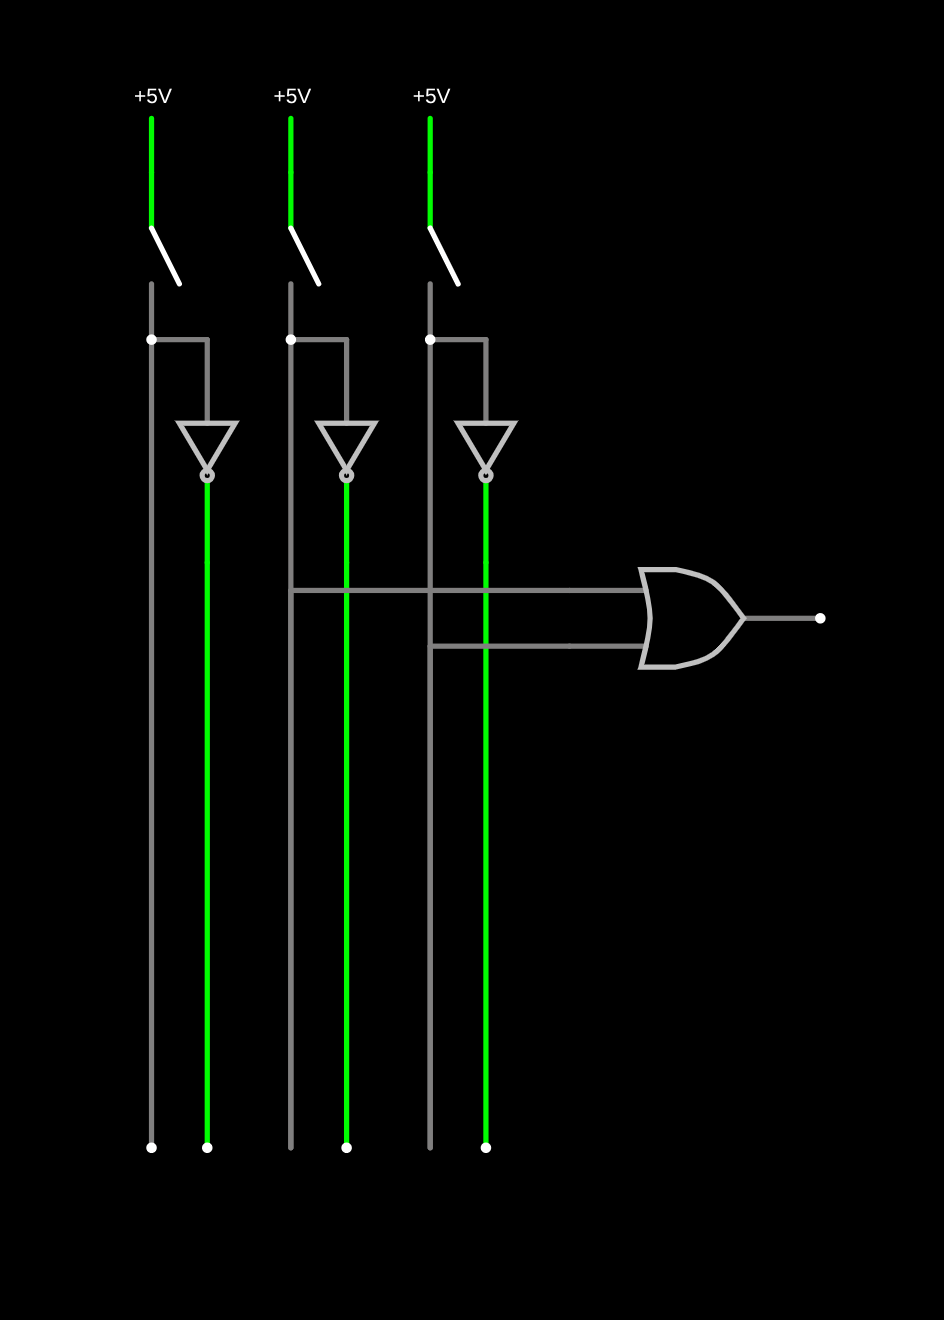
\includegraphics[width=0.6\textwidth]{img/Falstad/ej2.png}
    \caption{Simulación de la función en Falstad}
\end{figure}

\subsection{Descripción en Verilog}

\begin{Verbatim}[ frame=single, fontsize=\small, baselinestretch=1.2 ]
module ej2 (
    input x,
    input y,
    input z,
    output F
);

assign F = y | z;

endmodule
\end{Verbatim}

\subsection{Captura del RTL}
\begin{figure}[H]
    \centering
    
\includegraphics[width=0.8\textwidth]{img/Xilinx/ej2.png}
    \caption{Captura del RTL en Xilinx}
\end{figure}
\section{Ejercicio 3}

$$
F(x,y,z) = \sum(0,2,4,6)
$$

\subsection{Expresión mínima}

\begin{figure}[H]
    \centering
    \begin{karnaugh-map}[2][4][1][$z$][$y$][$x$]
        \centering
        \minterms{0,2,4,6}
        \implicant{0}{4}
    \end{karnaugh-map}
    \caption{Mapa de Karnaugh para la función}
\end{figure}

$$
F(x,y,z) = \overline{z}
$$

\subsection{Simulación en Falstad}
\begin{figure}[H]
    \centering
    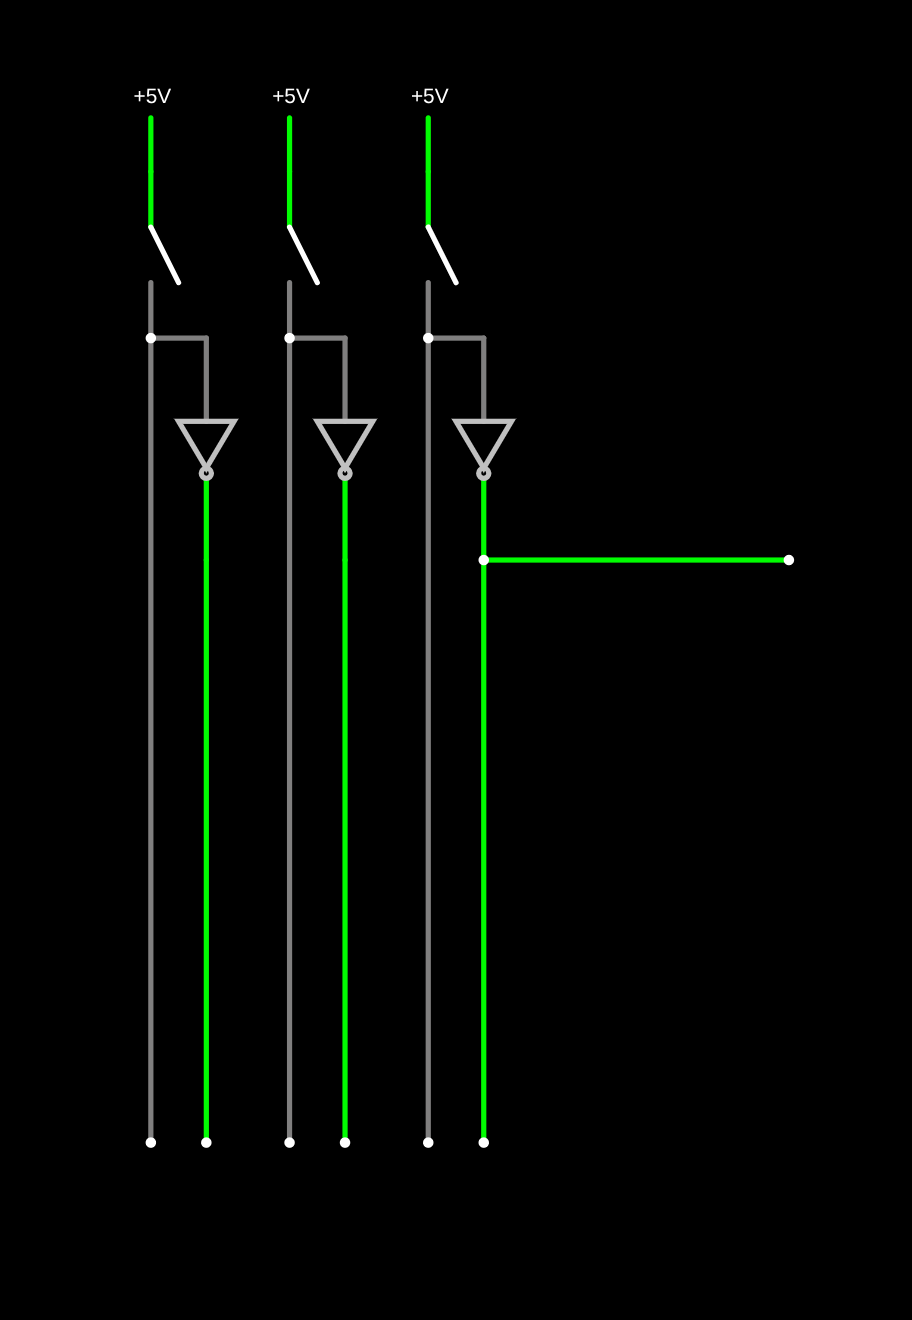
\includegraphics[width=0.6\textwidth]{img/Falstad/ej3.png}
    \caption{Simulación de la función en Falstad}
\end{figure}

\subsection{Descripción en Verilog}

\begin{Verbatim}[ frame=single, fontsize=\small, baselinestretch=1.2 ]
module ej3 (
    input x,
    input y,
    input z,
    output F
);

assign F = ~z;

endmodule
\end{Verbatim}

\subsection{Captura del RTL}
\begin{figure}[H]
    \centering
    
\includegraphics[width=0.8\textwidth]{img/Xilinx/ej3.png}
    \caption{Captura del RTL en Xilinx}
\end{figure}
\section{Ejercicio 4}

$$
F(x,y,z) = \sum(3,4,5,6,7)
$$

\subsection{Expresión mínima}

\begin{figure}[H]
    \centering
    \begin{karnaugh-map}[2][4][1][$z$][$y$][$x$]
        \centering
        \minterms{3,4,5,6,7}
        \implicant{6}{5}
        \implicant{3}{7}
    \end{karnaugh-map}
    \caption{Mapa de Karnaugh para la función}
\end{figure}

$$
F(x,y,z) = x + yz
$$

\subsection{Simulación en Falstad}
\begin{figure}[H]
    \centering
    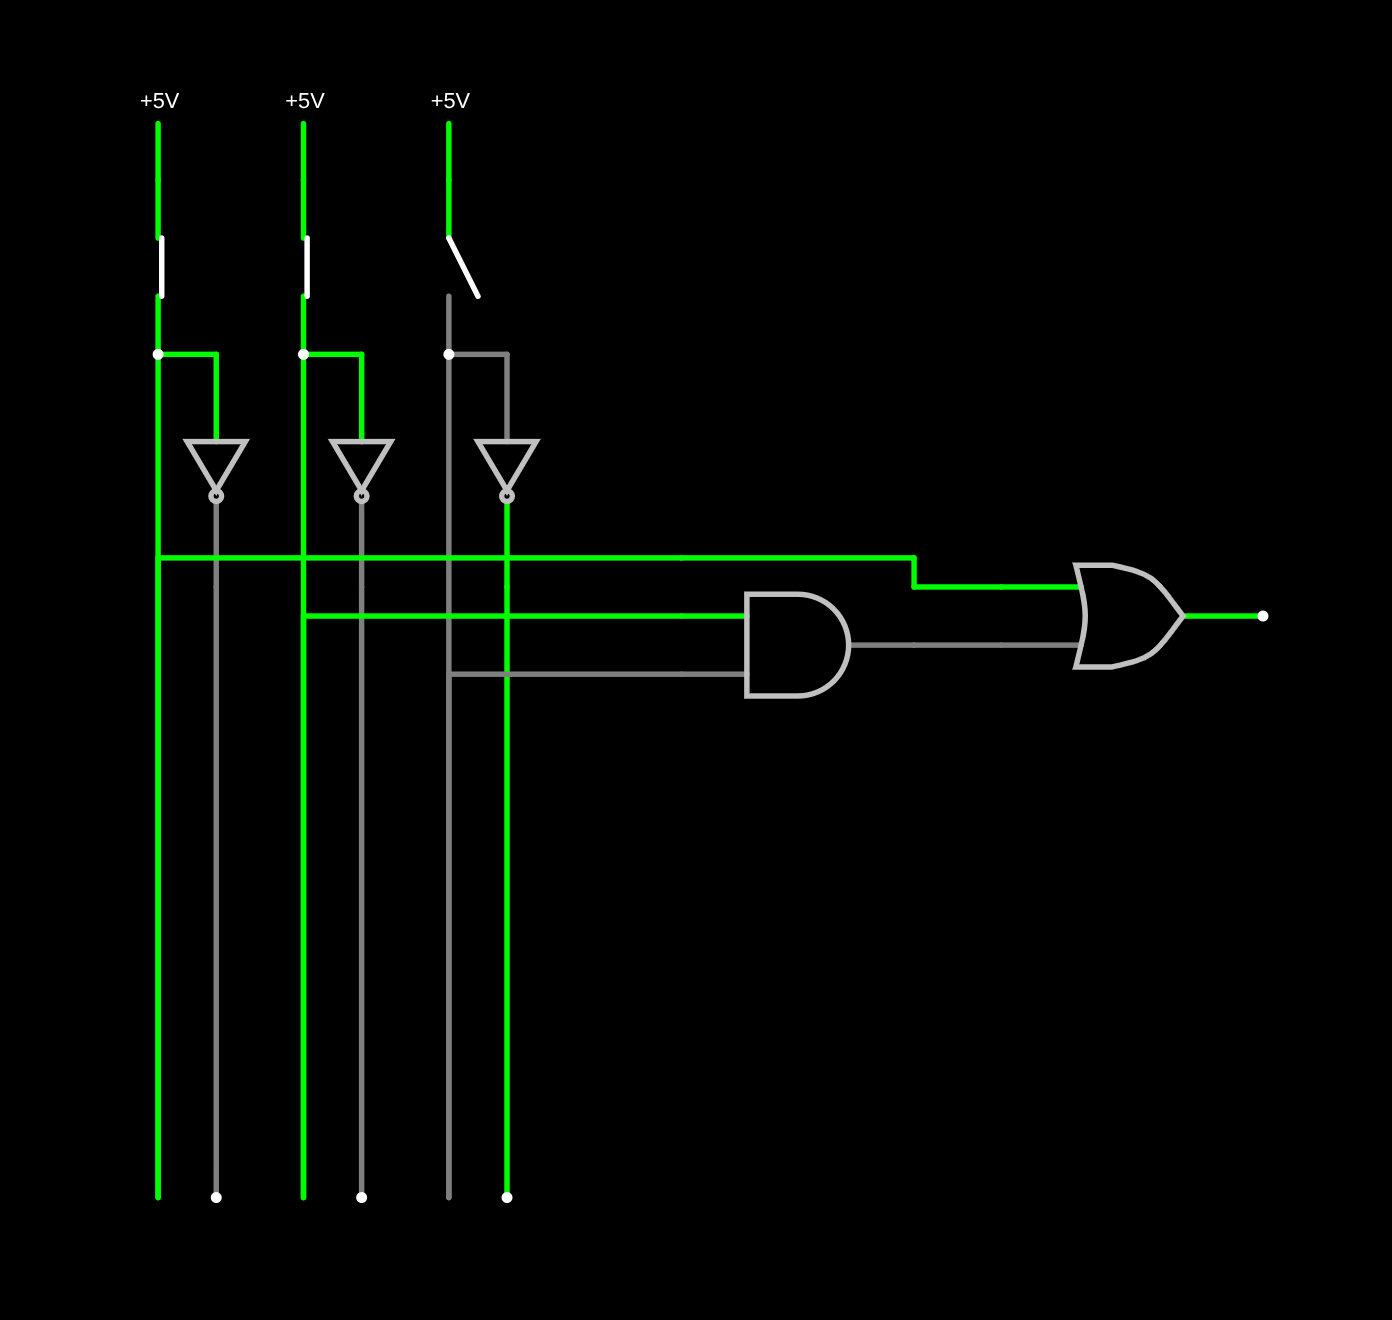
\includegraphics[width=0.6\textwidth]{img/Falstad/ej4.png}
    \caption{Simulación de la función en Falstad}
\end{figure}

\subsection{Descripción en Verilog}

\begin{Verbatim}[ frame=single, fontsize=\small, baselinestretch=1.2 ]
module ej4 (
    input x,
    input y,
    input z,
    output F
);

assign F = x | y & z;

endmodule
\end{Verbatim}

\subsection{Captura del RTL}
\begin{figure}[H]
    \centering
    
\includegraphics[width=0.8\textwidth]{img/Xilinx/ej4.png}
    \caption{Captura del RTL en Xilinx}
\end{figure}
\section{Ejercicio 5}

$$
F(A,B,C,D) = \sum(3,7,11,13,14,15) \, , \, X = 6,2
$$

\subsection{Expresión mínima}

\begin{figure}[H]
    \centering
    \begin{karnaugh-map}[4][4][1][$D$][$C$][$B$][$A$]
        \minterms{3,7,11,13,14,15}
        \terms{6,2}{X}
        \implicant{3}{11}
        \implicant{7}{14}
        \implicant{13}{15}
    \end{karnaugh-map}
    \caption{Mapa de Karnaugh para la función}
\end{figure}

$$
F(A,B,C,D) = BC+CD+ABD
$$

\subsection{Simulación en Falstad}
\begin{figure}[H]
    \centering
    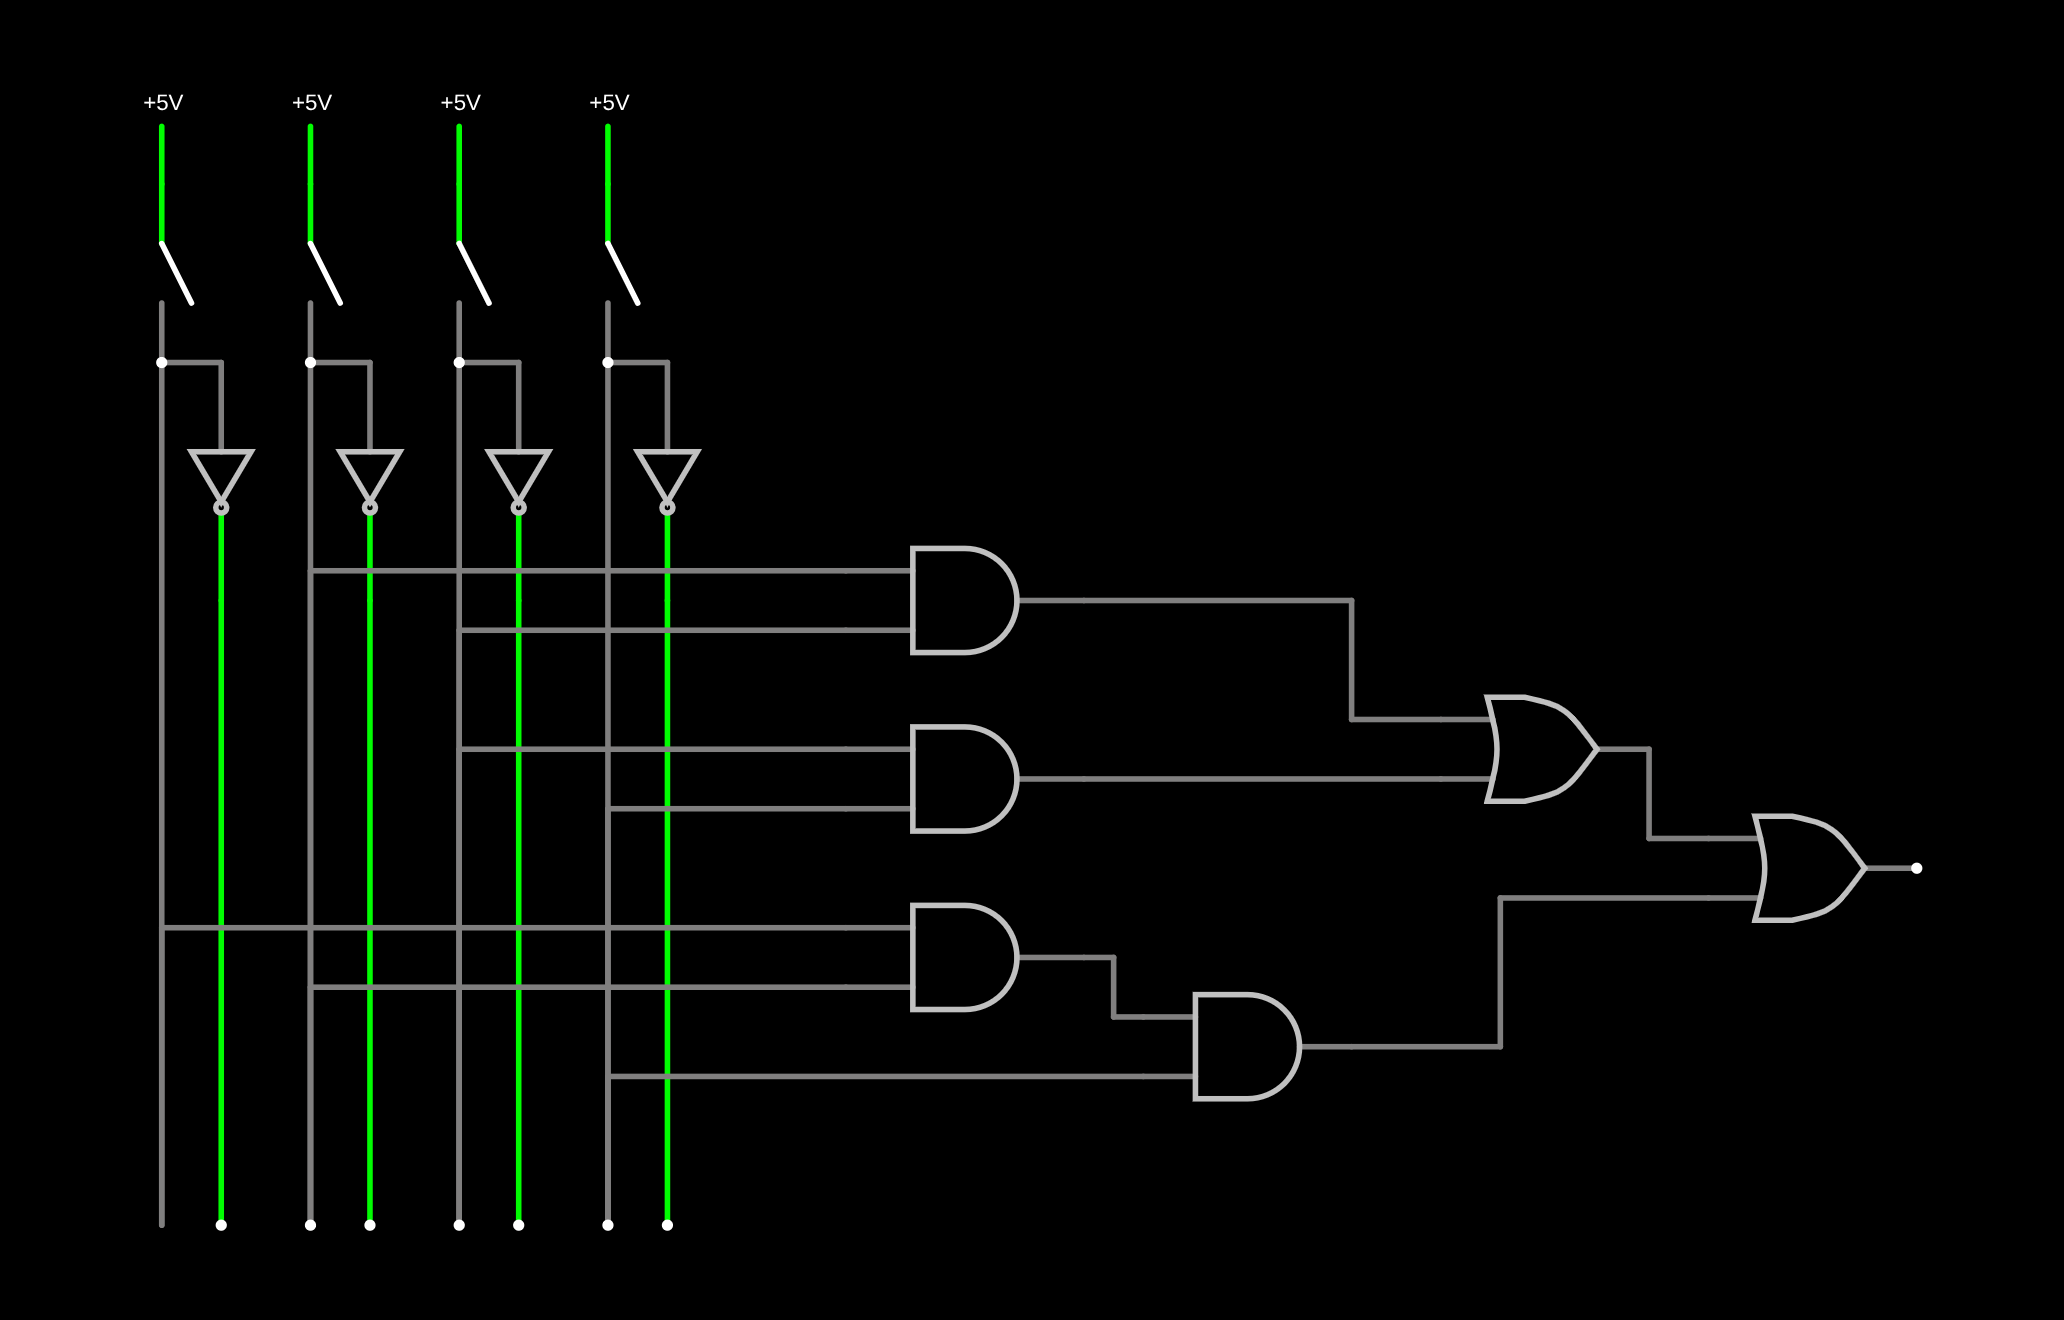
\includegraphics[width=0.6\textwidth]{img/Falstad/ej5.png}
    \caption{Simulación de la función en Falstad}
\end{figure}

\subsection{Descripción en Verilog}

\begin{Verbatim}[ frame=single, fontsize=\small, baselinestretch=1.2 ]
module ej5 (
    input A,
    input B,
    input C,
    input D,
    output F
);

assign F = B&C | C&D | A&B&D;

endmodule
\end{Verbatim}

\subsection{Captura del RTL}
\begin{figure}[H]
    \centering
    
\includegraphics[width=0.8\textwidth]{img/Xilinx/ej5.png}
    \caption{Captura del RTL en Xilinx}
\end{figure}
\section{Ejercicio 6}

$$
F(w,x,y,z) = \sum(2,3,12,13,14,15)\; , \; X = 6,7,10,11
$$

\subsection{Expresión mínima}

\begin{figure}[H]
    \centering
    \begin{karnaugh-map}[4][4][1][$z$][$y$][$x$][$w$]
        \minterms{2,3,12,13,14,15}
        \terms{6,7,10,11}{X}
        \implicant{3}{10}
        \implicant{12}{14}
    \end{karnaugh-map}
    \caption{Mapa de Karnaugh para la función}
\end{figure}

$$
F(w,x,y,z) = wx + y
$$

\subsection{Simulación en Falstad}
\begin{figure}[H]
    \centering
    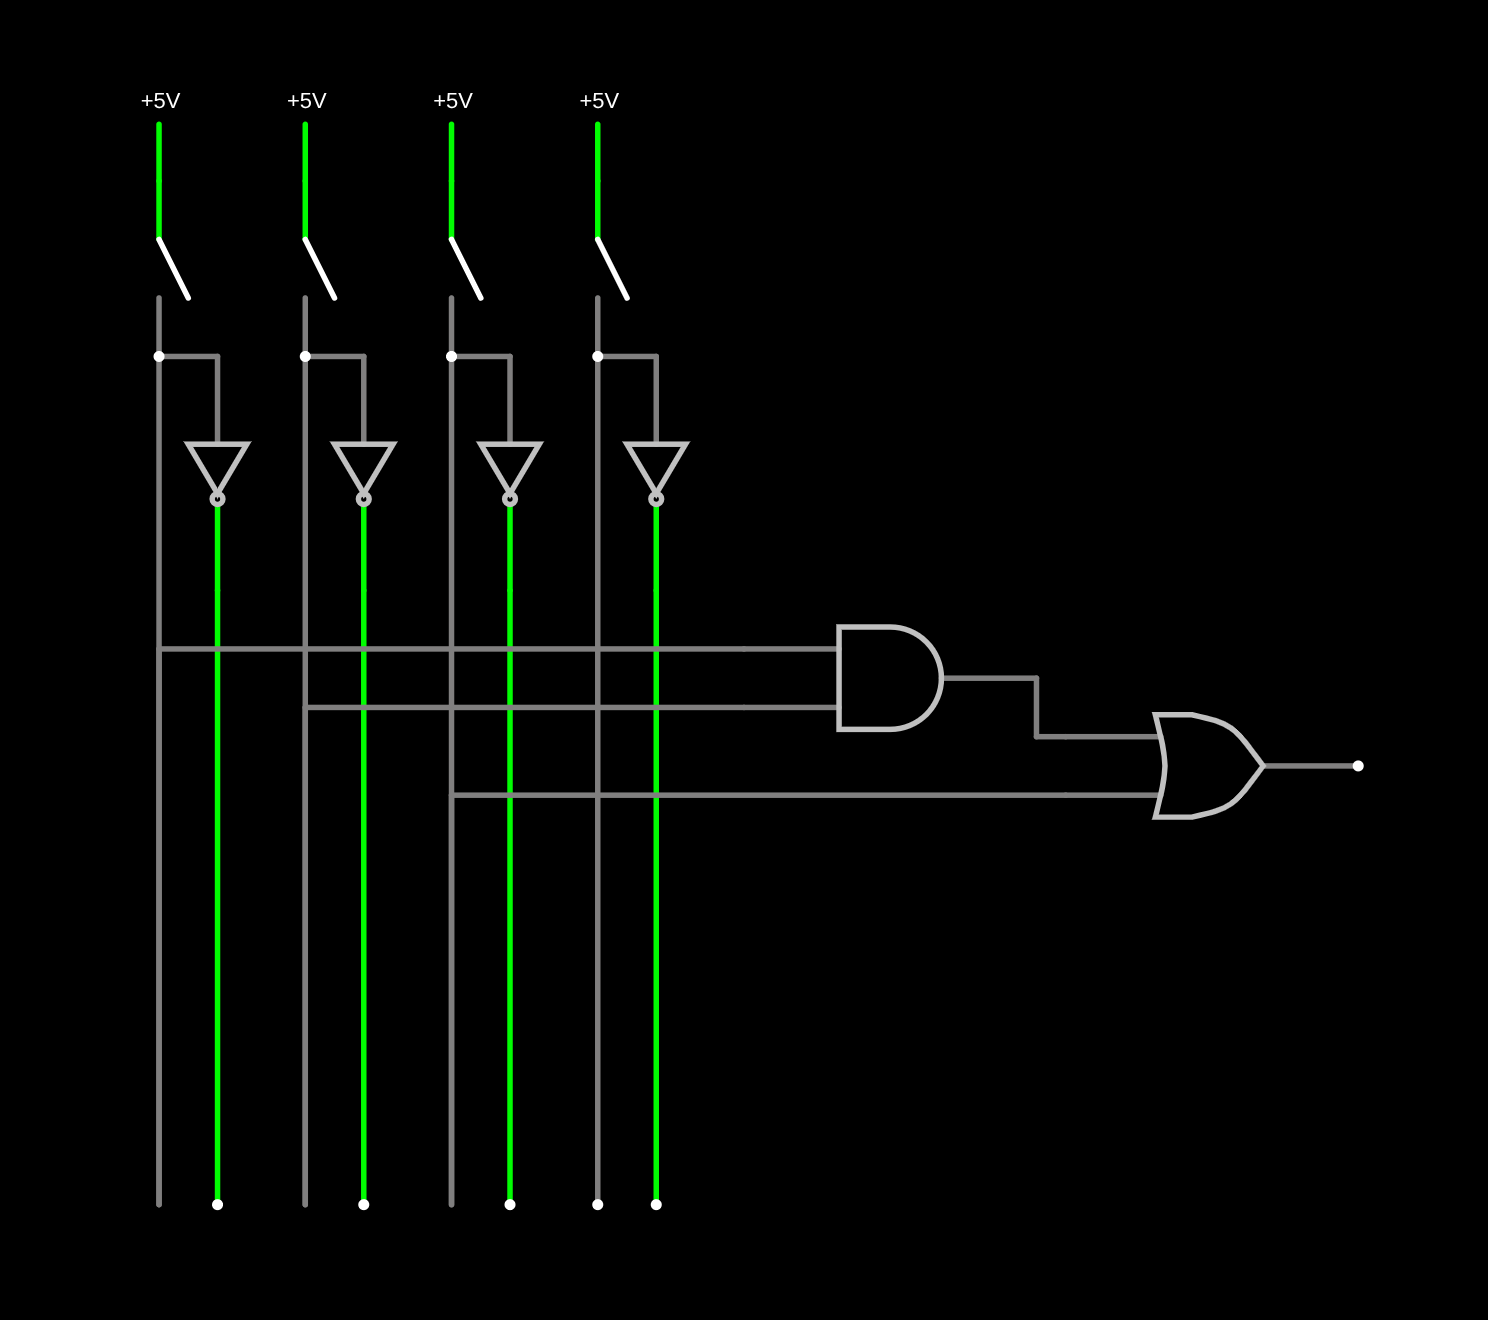
\includegraphics[width=0.6\textwidth]{img/Falstad/ej6.png}
    \caption{Simulación de la función en Falstad}
\end{figure}

\subsection{Descripción en Verilog}

\begin{Verbatim}[ frame=single, fontsize=\small, baselinestretch=1.2 ]
module ej6 (
    input w,
    input x,
    input y,
    input z,
    output F
);

assign F = w&x | y;

endmodule
\end{Verbatim}

\subsection{Captura del RTL}
\begin{figure}[H]
    \centering
    
\includegraphics[width=0.8\textwidth]{img/Xilinx/ej6.png}
    \caption{Captura del RTL en Xilinx}
\end{figure}
\section{Ejercicio 5}

$$
F(A,B,C,D) = \prod(1,3,5,7,13,15)
$$

\subsection{Expresión mínima}

\begin{figure}[H]
    \centering
    \begin{karnaugh-map}[4][4][1][$D$][$C$][$B$][$A$]
        \maxterms{1,3,5,7,13,15}
        \implicant{1}{7}
        \implicant{5}{15}
    \end{karnaugh-map}
    \caption{Mapa de Karnaugh para la función}
\end{figure}

\begin{align*}
F(A,B,C,D) &= (A+\overline{D})(\overline{B}+\overline{D})\\
F(A,B,C,D) &= A\overline{B} + \overline{D} 
\end{align*}

\subsection{Simulación en Falstad}
\begin{figure}[H]
    \centering
    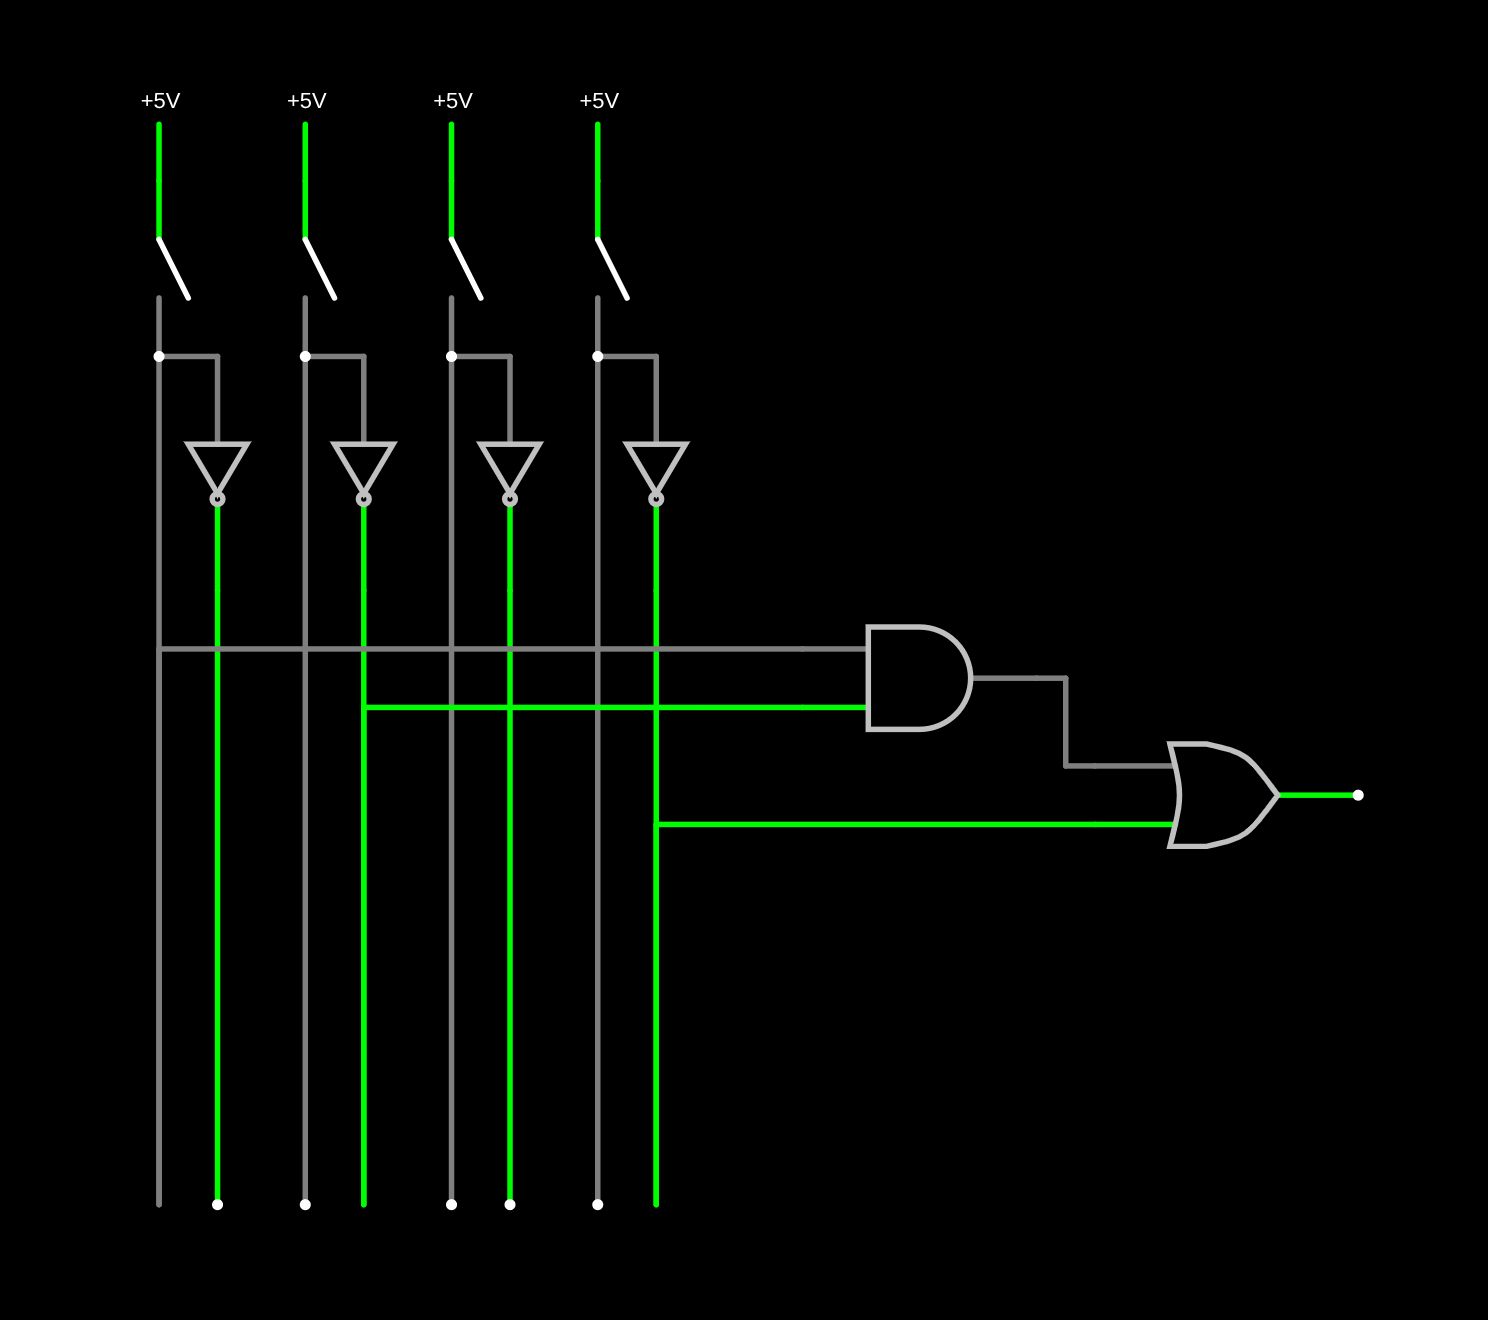
\includegraphics[width=0.6\textwidth]{img/Falstad/ej7.png}
    \caption{Simulación de la función en Falstad}
\end{figure}

\subsection{Descripción en Verilog}

\begin{Verbatim}[ frame=single, fontsize=\small, baselinestretch=1.2 ]
module ej5 (
    input A,
    input B,
    input C,
    input D,
    output F
);

assign F = A & ~B | ~D ;

endmodule
\end{Verbatim}

\subsection{Captura del RTL}
\begin{figure}[H]
    \centering
    
\includegraphics[width=0.8\textwidth]{img/Xilinx/ej7.png}
    \caption{Captura del RTL en Xilinx}
\end{figure}
\section{Ejercicio 5}

$$
F(A,B,C,D) = \prod(0,1,4,6,7,8,9,13,15)
$$

\subsection{Expresión mínima}

\begin{figure}[H]
    \centering
    \begin{karnaugh-map}[4][4][1][$D$][$C$][$B$][$A$]
        \maxterms{0,1,4,6,7,8,9,13,15}
        \minterms{2,3,5,10,11,12,14}
        \implicant{5}{5}
        \implicantedge{12}{12}{14}{14}
        \implicantedge{3}{2}{11}{10}
    \end{karnaugh-map}
    \caption{Mapa de Karnaugh para la función}
\end{figure}

$$
F(A,B,C,D) = \overline{B}C + \overline{A}B\overline{C}D + AB\overline{D}
$$

\subsection{Simulación en Falstad}
\begin{figure}[H]
    \centering
    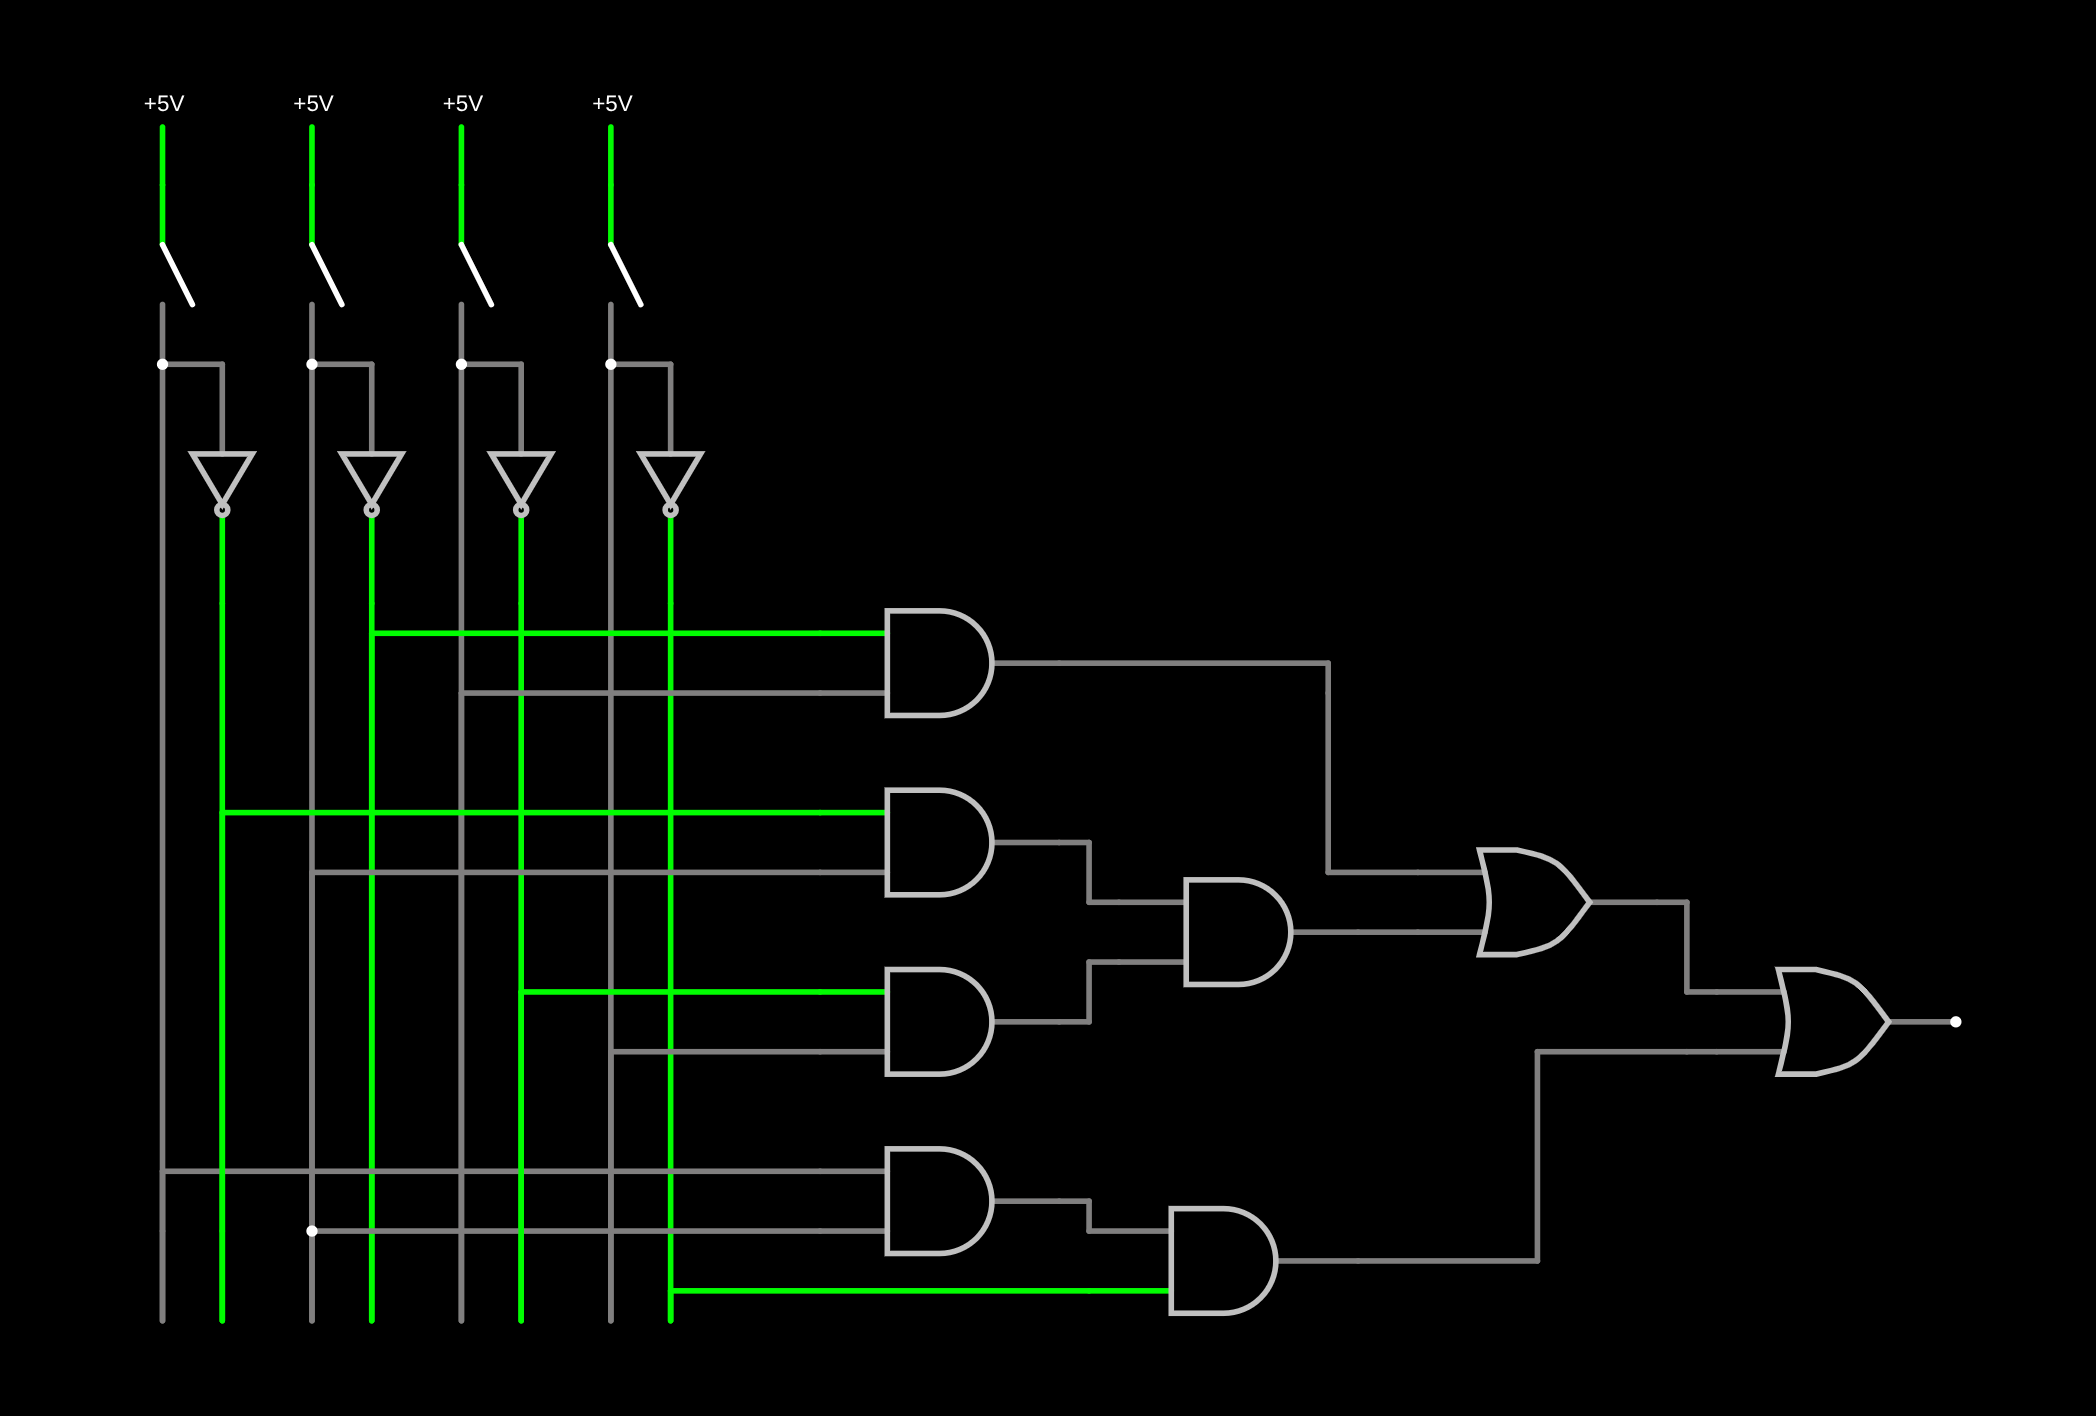
\includegraphics[width=0.6\textwidth]{img/Falstad/ej8.png}
    \caption{Simulación de la función en Falstad}
\end{figure}

\subsection{Descripción en Verilog}

\begin{Verbatim}[ frame=single, fontsize=\small, baselinestretch=1.2 ]
module ej8 (
    input A,
    input B,
    input C,
    input D,
    output F
);

assign F = ~B&C | ~A&B&~C&D | A&B&~D;

endmodule
\end{Verbatim}

\subsection{Captura del RTL}
\begin{figure}[H]
    \centering
    
\includegraphics[width=0.8\textwidth]{img/Xilinx/ej8.png}
    \caption{Captura del RTL en Xilinx}
\end{figure}

\end{document}